% Préambule commun des schémas TikZ (compilés séparément par construire_figures.py)
\documentclass[tikz,border=3pt]{standalone}
\usepackage[T1]{fontenc}
\usepackage[utf8]{inputenc}
\usepackage{lmodern}
\usepackage{amsmath,amssymb}
\usepackage{bm}
\usepackage[american,siunitx,straightvoltages]{circuitikz}
\usetikzlibrary{arrows.meta,positioning,calc,decorations.pathmorphing,
  decorations.markings,decorations.pathreplacing,patterns,shapes.geometric,
  shapes.misc,shapes.multipart,fit,backgrounds,3d,intersections,matrix}

\ctikzset{bipoles/length=1.1cm, amplifiers/scale=0.85, tripoles/op amp/width=1.4}

\tikzset{
  >={Latex[length=2mm,width=1.4mm]},
  every picture/.style={line width=0.6pt, font=\small},
  % schémas-blocs
  bloc/.style={draw, minimum width=1.5cm, minimum height=0.9cm, align=center,
               inner sep=3pt, fill=white},
  somme/.style={draw, circle, minimum size=4.5mm, inner sep=0pt, fill=white,
                path picture={\draw (path picture bounding box.north west)
                  -- (path picture bounding box.south east)
                  (path picture bounding box.north east)
                  -- (path picture bounding box.south west);}},
  gain/.style={draw, isosceles triangle, isosceles triangle apex angle=60,
               minimum size=8mm, inner sep=1pt, fill=white},
  bruit/.style={draw, circle, minimum size=4.5mm, inner sep=0pt, fill=white,
                path picture={\node at (path picture bounding box.center)
                  {\scriptsize$\ast$};}},
  cadre/.style={draw, dashed, rounded corners=1pt},
  cadrept/.style={draw, dash dot, rounded corners=1pt},
  fleche/.style={->},
  % mécanique
  bati/.style={pattern=north east lines, draw=none},
  ressort/.style={decorate, decoration={coil, aspect=0.4, segment length=2.2mm,
                  amplitude=2mm, pre length=2mm, post length=2mm}},
  zigzag/.style={decorate, decoration={zigzag, segment length=2mm,
                  amplitude=1.6mm, pre length=2mm, post length=2mm}},
  pivot/.style={draw, circle, fill=white, minimum size=2.2mm, inner sep=0pt},
  masse/.style={draw, fill=gray!25, minimum width=1.4cm, minimum height=0.8cm},
  cote/.style={<->, line width=0.4pt},
  axe/.style={->, line width=0.6pt},
  trait mixte/.style={dash dot, line width=0.4pt},
}

% Encastrement / bâti hachuré : \bati{(x1,y1)}{(x2,y2)} trace une ligne et ses hachures dessous
\newcommand{\bati}[3][0.18]{%
  \fill[pattern=north east lines] #2 rectangle ($#3+(0,-#1)$);
  \draw[line width=0.8pt] #2 -- #3;}

% Transducteur (deux cercles entrelacés) : \pic (t) at (x,y) {transducteur};  -> (t-o) entrée, (t-e) sortie
\tikzset{
  transducteur/.pic={\draw (-0.13,0) circle (0.24); \draw (0.13,0) circle (0.24);
    \coordinate (-o) at (-0.37,0); \coordinate (-e) at (0.37,0);
    \coordinate (-n) at (0,0.24); \coordinate (-s) at (0,-0.24);},
  bobine/.style={decorate, decoration={coil, aspect=0.7, segment length=1.4mm,
                 amplitude=1.6mm, pre length=1mm, post length=1mm}},
  sourcebruit/.style={draw, circle, minimum size=5mm, inner sep=0pt, fill=white,
                 label={[inner sep=0pt]center:$\ast$}},
  sourcecourant/.style={draw, circle, minimum size=5mm, inner sep=0pt, fill=white,
                 label={[inner sep=0pt]center:$\circledast$}},
}

% Composants compacts (pour les petits boîtiers des schémas-blocs)
\newcommand{\resistance}[2]{% de #1 à #2 (quelconque)
  \draw #1 -- ($#1!0.22!#2$) ($#1!0.78!#2$) -- #2;
  \draw[decorate, decoration={zigzag, segment length=1.5mm, amplitude=1.1mm}]
    ($#1!0.22!#2$) -- ($#1!0.78!#2$);}
\newcommand{\condensateur}[2]{% horizontal de #1 à #2
  \draw #1 -- ($($#1!0.5!#2$)+(-0.05,0)$) ($($#1!0.5!#2$)+(0.05,0)$) -- #2;
  \draw[line width=1pt] ($($#1!0.5!#2$)+(-0.05,0.14)$) -- ($($#1!0.5!#2$)+(-0.05,-0.14)$)
                        ($($#1!0.5!#2$)+(0.05,0.14)$) -- ($($#1!0.5!#2$)+(0.05,-0.14)$);}
% R // C horizontal : \RparC{(x,y)}{longueur}{écart}  (centre, longueur totale, écart vertical)
\newcommand{\RparC}[3]{%
  \coordinate (rcA) at ($#1+(-#2/2,0)$); \coordinate (rcB) at ($#1+(#2/2,0)$);
  \draw (rcA) -- ++(0.15,0) coordinate (rcA1) (rcB) -- ++(-0.15,0) coordinate (rcB1);
  \draw (rcA1) -- ++(0,#3/2) (rcA1) -- ++(0,-#3/2) (rcB1) -- ++(0,#3/2) (rcB1) -- ++(0,-#3/2);
  \resistance{($(rcA1)+(0,#3/2)$)}{($(rcB1)+(0,#3/2)$)}
  \condensateur{($(rcA1)+(0,-#3/2)$)}{($(rcB1)+(0,-#3/2)$)}}

\begin{document}
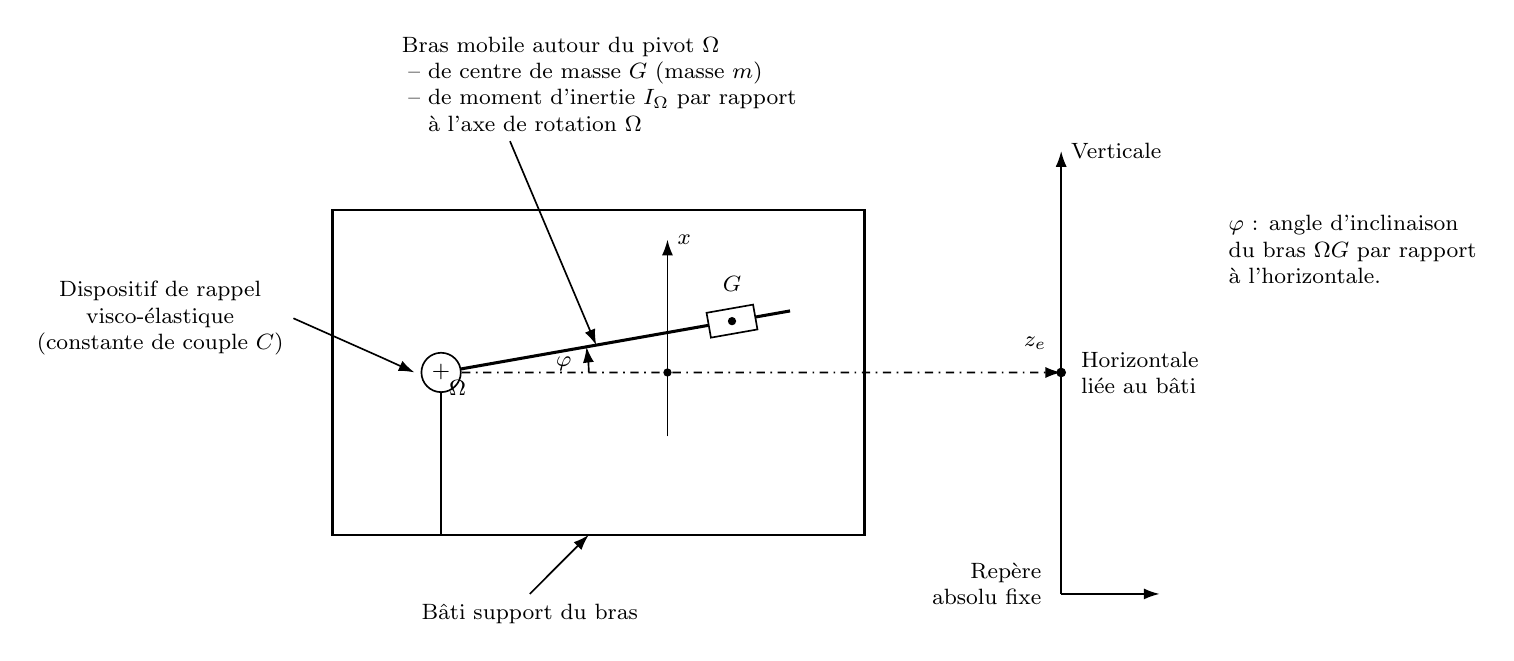
\begin{tikzpicture}[font=\footnotesize, scale=1.25]
  % bâti
  \draw[line width=1pt] (0,0) rectangle (5.4,3.3);
  \coordinate (O) at (1.1,1.65);
  \draw (O) -- (O |- 0,0);
  % horizontale liée au bâti
  \draw[dash dot, ->] (O) -- (7.4,1.65);
  % bras incliné de phi
  \coordinate (G) at ($(O)+(10:3.0)$);
  \draw[line width=1.1pt] (O) -- ($(O)+(10:3.6)$);
  \node[draw, fill=white, minimum width=6mm, minimum height=3.2mm, rotate=10] at (G) {};
  \fill (G) circle (1.2pt);
  \node[above=2.5mm] at (G) {$G$};
  \draw[->] ($(O)+(0:1.5)$) arc (0:10:1.5);
  \node at ($(O)+(4:1.25)$) {$\varphi$};
  % axe sensible x
  \draw[axe] (3.4,1.0) -- (3.4,3.0) node[right] {$x$};
  \fill (3.4,1.65) circle (1.2pt);
  % pivot et dispositif de rappel
  \node[pivot, minimum size=5mm] at (O) {};
  \node at (O) {$+$};
  \node[below right=-1pt] at (O) {$\Omega$};
  % repère absolu
  \draw[axe] (7.4,-0.6) -- (7.4,3.9) node[right] {Verticale};
  \fill (7.4,1.65) circle (1.4pt);
  \node[left] at (7.35,1.95) {$z_e$};
  \node[right, align=left] at (7.5,1.65) {Horizontale\\liée au bâti};
  \draw[axe] (7.4,-0.6) -- (8.4,-0.6);
  \node[left, align=right] at (7.3,-0.5) {Repère\\absolu fixe};
  % légendes
  \node[align=left, anchor=south west] (bras) at (0.6,4.0)
    {Bras mobile autour du pivot $\Omega$\\
     \;-- de centre de masse $G$ (masse $m$)\\
     \;-- de moment d'inertie $I_\Omega$ par rapport\\
     \;\phantom{--} à l'axe de rotation $\Omega$};
  \draw[->] (1.8,4.0) -- ($(O)+(10:1.6)$);
  \node[align=center, anchor=east] (rap) at (-0.4,2.2)
    {Dispositif de rappel\\visco-élastique\\(constante de couple $C$)};
  \draw[->] (rap.east) -- ++(0.9,-0.4) -- ($(O)+(-0.27,0)$);
  \node[anchor=north] (bati) at (2.0,-0.6) {Bâti support du bras};
  \draw[->] (bati.north) -- (2.6,0);
  \node[align=left, anchor=west] at (9.0,2.9)
    {$\varphi$ : angle d'inclinaison\\du bras $\Omega G$ par rapport\\à l'horizontale.};
\end{tikzpicture}
\end{document}
